\chapter{Evaluation}
\label{chapter:Evaluation}

This section experimentally answers the following questions:

\begin{itemize}

%\item
%  Is our confidentiality specifications trustworthy?  That is, are noninterference theorems sufficient for applications to prove confidentiality of their own data?
%  What assumptions do these proofs rely on?

\item
  How much effort was required to develop the frameworks, and to use frameworks to prove the security of the systems?

\item 
  How are the performances of the systems compare to existing ones?
  %How much runtime overhead does DiskSec's approach impose in SFSCQ?
\end{itemize}

\section{Specification trustworthiness}

To evaluate the trustworthiness of SFSCQ's specifications, we performed several
analyses.


\paragraph{End-to-end application confidentiality.}

To demonstrate that SFSCQ's specifications capture confidentiality in
a useful way, we developed a simple application on top of SFSCQ that
copies a file, wrote a confidentiality specification for this application
(namely, that the application does not leak the data of the copied
file), and proved it.  This application tests two aspects of SFSCQ's
specs.  The first is, does SFSCQ's specification actually guarantee
confidentiality?  The second has to do with SFSCQ's discretionary access
control model: can application developers demonstrate that they are not
inadvertently leaking data, despite having the discretion to do so?

We were able to prove the correctness and security of our implementation
of \texttt{cp}.  This suggests that SFSCQ's specifications capture sufficient
information for \texttt{cp} to conclude that its data remains confidential,
and that it is possible for application developers to show that they do
not abuse their discretionary privileges by leaking data.


\paragraph{Bug case study.}

To evaluate whether SFSCQ's specifications would eliminate real
security bugs, we qualitatively analyzed the bugs presented in
\ref{s:motivation} to determine whether SFSCQ's theorems preclude
the possibility of that bug.  \ref{fig:bugs-addressed} shows the
results.  Functional correctness theorems preclude the possibility of
integrity bugs.  DiskSec state noninterference precludes the possibility
of all confidentiality bugs in our study.  No bugs were prevented by
return-value noninterference, because return-value noninterference captures a
particularly simple kind of bug, such as the file system forgetting
to check the ACL on \texttt{open()}.  No file-system developers made this
mistake in our study.  Nonetheless, return noninterference is important
for completeness of SFSCQ's theorems.  Overall, the results demonstrate
that SFSCQ's theorems preclude the possibility of all studied bugs.

\begin{figure}[H]
  \centering
  \small
  \begin{tabular}{| l | c | c |}
    \hline
    \textbf{Description} & \textbf{Theorem}  & \textbf{violated}\\
    \hline
    anyone can change POSIX ACLs~\cite{CVE-2010-2071, CVE-2010-1641, CVE-2016-1237} & state NI & \\
    reiserfs permissions can be changed by writing to hidden file~\cite{CVE-2010-1146} & state NI & \\
    truncated data can be accessed~\cite{CVE-2015-8374} & state NI  &\\
    crash can expose deleted data in ext4~\cite{CVE-2017-7495} & state NI  &\\
    crash can expose data in ext4~\cite{git:469017} & state NI  &\\
    can overwrite append-only file in ext4, btrfs~\cite{CVE-2010-2066, CVE-2010-2537} & integrity  &\\
    can overwrite arbitrary files in ext4~\cite{CVE-2009-4131} & integrity & \\
    % SGID directories can become writeable in overlayfs~\cite{CVE-2016-1575} &
    % write confidentiality, but \emph{N/A}\footnote{any SGID, writeable
    % directory violates write confidentiality, but no support or model of
    % SUID/SGID} \\
    \hline
  \end{tabular}
  \caption{Security bugs in Linux file systems and which SFSCQ theorem precludes them.}
  \label{fig:bugs-addressed}
\end{figure}


\paragraph{Trusted computing base.}

Both systems assume the correctness of several components.  They assume
that Coq's proof checking kernel is correct, because it verifies
the proofs. Both systems assume that the Haskell runtime and support
libraries (and the underlying Linux kernel) do not have bugs, since
they generate executable code through extraction to Haskell. Both systems
assume that their respective framework's model of the disk is accurate.  In particular, all
non-determinism in the oracles and execution semantics must be ``realizable,''
in the sense that it is actually possible for an execution to observe
all specified non-determinism (e.g., crashing at any point), and this
non-determinism must be independent of confidential data.  All proofs in the frameworks and the systems are checked by Coq proof assistant.


\section{Effort}

% these numbers were computed by the scripts in
% osdi18-security/effort-estimate/; see the README.md there for details.

To understand how much effort was required to verify DiskSec and SFSCQ, we
compared SFSCQ to the implementation of DFSCQ on which SFSCQ is based.
\ref{fig:loc} shows the results (counting the sum of lines removed and lines
added), breaking down the differences into several categories.  The core
infrastructure, including improvements to DFSCQ's CHL, amounted to around
9,300 lines.  We made significant changes to DFSCQ to develop SFSCQ, but many
of these changes were mechanical fixes to proofs to address small changes. In
addition, using DiskSec in SFSCQ required around 1,900 lines of new code and proofs.
Porting DFSCQ to the first version of DiskSec (without support for changing
permissions) took one author about 3 months, and another 2 months to
mostly finish support for permission changes.

\begin{figure}[H]
  \centering
  \begin{tabular}{lr}
    \hline
    \textbf{Component} & \textbf{Changes to DFSCQ} \\
    \hline
    DiskSec & 9,283 \\
    DFSCQ proof fixes & $-10,471$, $+26,433$ \\
    & \quad (36,094 total) \\
    SFSCQ impl.\ and proofs & 1,837 \\
    Verified \texttt{cp} application & 407 \\
    \hline
  \end{tabular}
  \caption{Lines of code change required to implement DiskSec and apply it to build
    SFSCQ. Counts measure the diff between DFSCQ and SFSCQ.}
  \label{fig:loc}
\end{figure}


\section{Performance}
We conducted two experiments to measure the performance of our file systems: (1) performance comparison between SFSCQ and DFSCQ, (2) performance comparison between ConFs and FSCQ. We chose reference file systems to be as similar as possible to our file systems. 
DFSCQ was a natural one for the SFSCQ, since SFSCQ is a modified version of the DFSCQ. We used FSCQ for ConFs because it is more similar to ConFs than SFSCQ or DFSCQ.

\paragraph{SFSCQ Performance}
We expect that the performance overhead of DiskSec is nearly zero, because
most of its code changes (such as handles, sealing, and unsealing) are
eliminated in the process of generating executable code.  (All of the
Seal and Unseal operations turn into \texttt{return} statements.)  The only
exception is checking permissions when reading data from a file; the
original DFSCQ implementation had no permission checks, which we added
in SFSCQ.

To check that DiskSec introduces almost no overhead,
we used two microbenchmarks (LFS smallfile and largefile
benchmarks~\cite{rosenblum:lfs} as modified by DFSCQ~\cite{chen:dfscq}).
As a baseline, we compare with two versions of DFSCQ, on which SFSCQ
is based.  The first is unmodified DFSCQ\@.  The second is a version of
DFSCQ with a two-disk-barrier write-ahead log (instead of its default
checksum-based log).  This matches the modification we made to SFSCQ, as
mentioned in \ref{s:fs:impl}.  For comparison with other file systems,
such as Linux ext4, we refer the reader to the detailed evaluation in
the DFSCQ paper~\cite[\S 7.4]{chen:dfscq}.

\ref{fig:perf} shows the results, which confirm that SFSCQ performs
nearly identically to DFSCQ in the same logging configuration.  The use
of a two-disk-barrier write-ahead log incurs some performance overhead
for smallfile; largefile performance is not impacted because its file
data writes bypass the log.

\begin{figure}[H]
  \centering
  \begin{tabular}{lrr}
    \hline
    \textbf{Filesystem} & \textbf{smallfile} & \textbf{largefile} \\
    \hline
    DFSCQ & 446 files/s & 108 MB/s \\
    DFSCQ (no checksums) & 295 files/s & 109 MB/s \\
    SFSCQ & 299 files/s & 100 MB/s \\
    \hline
  \end{tabular}
  \caption{Benchmarks showing performance of SFSCQ compared to DFSCQ and a
    version of DFSCQ with a comparable logging implementation.  Numbers
    shown are the median of 30 runs.}
  \label{fig:perf}
\end{figure}


\paragraph{ConFs Performance}
To measure the performance of ConFs, we used four microbenchmarks (LFS smallfile, largefile, rename, and createdelete
benchmarks~\cite{rosenblum:lfs} as modified by DFSCQ~\cite{chen:dfscq}). We compared ConFs against FSCQ and SFSCQ where we ran each benchmark 10 times and take their average. In our experiments, ConFs achieved 60\% of FSCQ's performance in smallfile, 82\% in rename, and 52\% in createdelete benchmarks. In largefile benchmark, ConFs achieved 83\% of FSCQ's performance in makefile test and 284\% in writefile test. Figure \ref{fig:Performance_Comparison} and \ref{fig:Performance_Comparison_Largfile} demonstrate the results. We include performance numbers for SFSCQ for the sake of completeness, although it performs an order of magnitude better due to being more optimized for performance.

\begin{figure}[H]
         \centering
          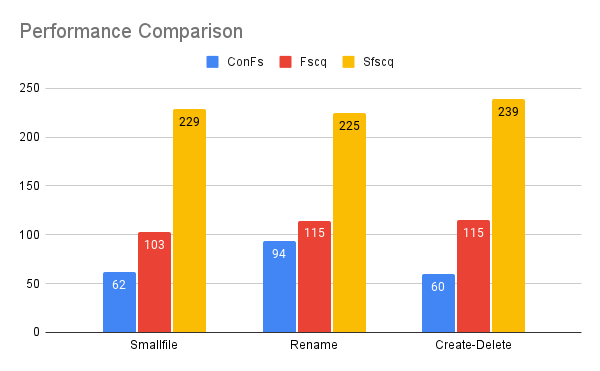
\includegraphics[scale=0.5]{templates/figures/Performance Comparison.png}
    \caption{Performance comparison for smallfile, rename and createdelete benchmarks.}
    \label{fig:Performance_Comparison}
\end{figure}

\begin{figure}[H]
    \centering
    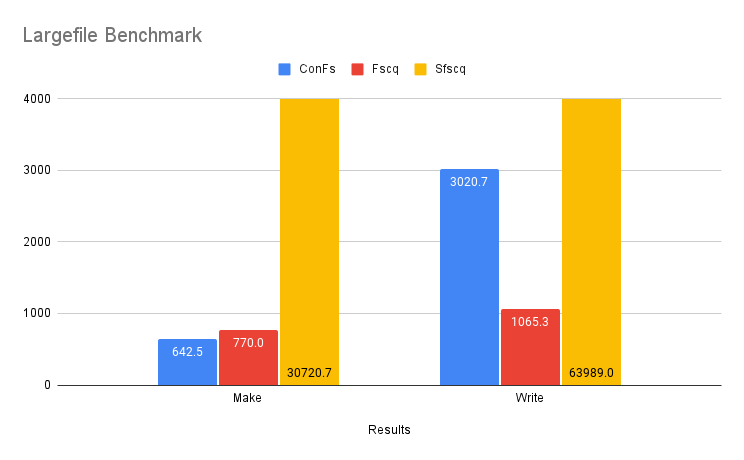
\includegraphics[scale=0.5]{templates/figures/Largefile Benchmark.png}
    \caption{Performance comparison for the largefile benchmark.}
    \label{fig:Performance_Comparison_Largfile}
\end{figure}

Since ConFs isn't build with performance in mind, it lacks many optimizations that can increase its performance. Most impactful of those is a buffer cache to keep recent disk reads and writes in the memory for faster access. Absence of the buffer cache resulted in many disk read operations (e.g., allocator bitmaps, log header, etc.) to be executed per system call. This introduced a significant performance overhead to the system. 

\begin{figure}[H]
    \centering
    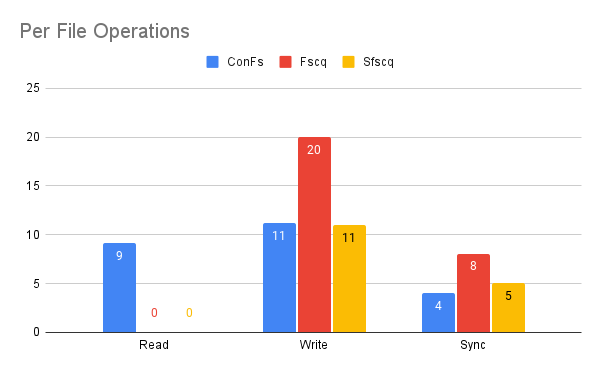
\includegraphics[scale=0.5]{templates/figures/Per File Operations.png}
    \caption{Per-file disk operations in smallfile benchmark.}
    \label{fig:Smallfile_Per_File_benchmark}
\end{figure}

We can see that ConFs' slowdown comes from disk reads in per-file disk operations breakdown of smallfile benchmark, displayed in figure  \ref{fig:Smallfile_Per_File_benchmark}. Even though ConFs makes less disk writes and syncs than FSCQ, 9 extra reads lead to a worse performance. Similarly, ConFs performs significantly better than FSCQ in writefile test because test is dominated by write operations.\\

\noindent
\textbf{ConFrm effort numbers:}\\
Supplementary Libs (listutils, mem, totalmem): 7647 cloc\\
ConFrm : 3407 cloc\\
\noindent
\textbf{ConFs effort numbers:}\\
Implementation + Functional Correctness : 16852 cloc\\
Refinements: 4594 cloc\\
Top Level NI : 1950 cloc\\
Simulations + Transfers: 18887 cloc\\
\noindent
\textbf{Grand Total:} 53405 cloc